\setlength{\parskip}{1em}

\chapter{Zadání}
Naprogramujte síťovou hru (server, klient) na protokolu TCP.

Úlohu naprogramujte v programovacím jazyku C/C++ anebo Java (C\#). Pokud se jedná o úlohu server/klient, pak klient bude v Javě (C\#) a server v C/C++. Komunikace bude realizována textovým nešifrovaným protokolem nad TCP protokolem. Výstupy serveru budou v alfanumerické podobě, klient může komunikovat i v grafice (není podmínkou). Server řešte pod operačním systémem Linux, klient může běžet pod OS Windows.

Realizujte konkurentní (paralelní) servery. Server musí být schopen obsluhovat požadavky více klientů souběžně. Bude možno hrát více her najednou a hru o větším počtu hráčů (dle pravidel hry). Klient se bude moct znovu připojit do přerušené hry.

Uživatelské rozhraní klienta bude nezávislé na zpoždění síťových operací. Aplikace se bude schopna vyrovnat s problémy na síti.


\chapter{Komunikační protokol}
Komunikační protokol pracuje na přenosu ASCII řetězců. Jednotlivé části jsou odděleny znakem ':' a hodnoty znakem ';'. Zpráva je zakončena '\textbackslash{n}'.

\section{Komunikace server-klient}
\begin{tabular}{|l|c|c|c|}
\hline
& Server & & Klient \\
\hline
Přihlášení & & \leftarrow & NICK \\
& NICKOK & \rightarrow & \\
& NICKERR & \rightarrow & \\
\hline
Znovu připojení do hry & RETURN & \rightarrow & \\
& & \leftarrow & RETURN \\
& & \leftarrow & NEW \\
\hline
Zahájení hry & GAME & \rightarrow & \\
& GAMER & \rightarrow & \\
\hline
Tahy & TURN & \rightarrow & \\
& & \leftarrow & TURN \\
& TURNOK & \rightarrow & \\
& TURNERR & \rightarrow & \\
Přeposlání tahu & TURNP & \rightarrow & \\
\hline
Ukončení hry & & \leftarrow & END \\
\hline
Hráč opustli hru/znovu se připojil & DISC & \rightarrow & \\
& RECN & \rightarrow & \\
\hline
Ping & & \leftarrow & PING \\
& PING & \rightarrow & \\
\hline
Chyba v přijaté zprávě  & & \leftarrow & ERR \\
& ERR & \rightarrow & \\

\hline
\end{tabular}

\section{Server -$>$ Klient}
\begin{tabular}{|l|p{5.1cm}|p{5cm}|}
\hline
Klíčové slovo & Předpis & Význam \\ \hline
NICKOK	& NICKOK	& Nick je přijat \\ \hline
NICKERR	& NICKERR:value	& Nick je nevalidní: USE - nick je obsazen / CHAR - nick obsahuje nevalidní znaky \\ \hline
GAME	& GAME:game\_ID:pl\_ID,nick; pl\_ID,nick;...	& Připojení do nové hry, info o hráčích \\ \hline
GAMER	& GAMER:game\_ID:pl\_ID,nick, score;pl\_ID,nick,score;...: x,y,char;x,y,char;...	& Připojení do existující hry, info o hráčích, info o tazích \\ \hline
TURN	& TURN	& Tah hráče \\ \hline
TURNP	& TURNP:pl\_ID:score;x,y,char; x,y,char;...	& Tah protihráče \\ \hline
TURNOK	& TURNOK	& Tah je přijat \\ \hline
TURNERR	& TURNERR	& Tah nebyl přijat \\ \hline
RETURN	& RETURN	& Hráč se může znovu připojit do opuštěné hry \\ \hline
DISC	& DISC:pl\_ID	& Hráč opustil hru \\ \hline
RECN	& RECN:pl\_ID	& Hráč se znovu připojil do hry \\ \hline
PING	& PING	& Odpověď na kontrolní zprávu od klienta \\ \hline
ERR	& ERR:value	& Chyba v přijaté zprávě \\ \hline
\end{tabular}

\section{Klient -$>$ Server}
\begin{tabular}{|l|p{5cm}|p{5cm}|}
\hline
Klíčové slovo & Předpis & Význam \\ \hline
NICK	& NICK:nick;n	& Připojení se do hry, nick a počet hráčů \\ \hline
TURN	& TURN:game\_ID:score; x,y,char;x,y,char;...	& Tah hráče \\ \hline
RETURN& RETURN 	& Vracení se do hry \\ \hline
NEW		& NEW	& Nová hra \\ \hline
END		& END	& Konec hry \\ \hline
PING	& PING	& Kontrolní zpráva, jestli je spojení se serverem \\ \hline
ERR		& ERR:value	& Chyba v přijaté zprávě \\ \hline
\end{tabular}



\chapter{Implementace}

\section{Server}

Server je implementován v jazyce C++.

O síťové spojení se stará třída \emph{Network}, o správu her a přidělování hráču pak třída \emph{GameManager}. Datová struktura pro hru a její ovládání je ve třídě \emph{Game}, datová struktura jednotlivých hráčů je třída \emph{Player}.

Po spuštění aplikace se vytvoří BSD socket, nabinduje se na zvolený port (defaultně 1993) a spustí se vlákno, které naslouchá příchozím spojením. Také se spustí vlákno čekající na příkazy z konzole.

Po připojení hráče se spustí se vlákno, které naslouchá příchozím zprávám od klienta, a vlákno, které kontroluje zda je spojení s klientem aktivní. Zkontroluje se, zda přezdívka již není použita a v případě, že je volná, klient se notifikuje o přijetí a přidá se do seznamu hráčů pro hru o zvoleném počtu hráčů (2, 3, 4). Pokud je přezdívka obsazena nebo nevalidní, je o tom hráč informován a musí použít jinou. Pokud je v seznamu pro danou hru určené množství hráčů, spustí se hra.

Hráči se ve svých tazích střídají. Hráči, je odeslána notifikace, že je na tahu. Hra poté čeká, až od hráče přijme jeho tah. Ten zvaliduje a uloží do dvourozměrného pole. Hráči pošle notifikaci o přijetí (či nepřijetí) tahu a ostatním hráčům tah přepošle. Poté notifikuje dalšího hráče na tahu.

Při odpojení nebo znovu připojení některého z hráčů server notifikuje všechny hrající hráče. Odpojený klient se může znovu připoji a má na výběr, zda se znovu připojí do rozehrané hry nebo chce hrát novou hru. Při znovu připojení se mu odešle aktuální stav hry. Pro hraní hry musí být připojeni minimálně 2 hráči.

Hra se ukončí v okamžiku, kdy se odpojí všichni hráči (jejich přezdívky jsou pak volné). Pokud od klienta dorazí zpráva, která neodpovídá komunikačnímu protokolu, je spojení s klientem ukončeno. Zadáním příkazu \emph{exit} se zavře socket a server se ukončí.

\section{Klient}

Klient je implementován v jazyce C\#, uživátělské rozhraní je implementováno knihovnou WinForms.

Aplikace má 2 uživatelská okna, jedno pro připojení ke hře a druhé k ovládání hry. O komunikaci se serverem se stará třída \emph{Network}. Datová struktura pro hru je třída \emph{Game} a datová struktura hráče je třída \emph{Player}.

Pro připojení musí být vyplněna IP adresa a port serveru, přezdívka hráče a zvolen počet hráčů. Poté se vytvoří socket a pokusí se přípojit k severu. Následně se na server odešle přezdívka a počet hráčů, spustí se vlákno, které naslouchá příchozím zprávám ze serveru, a vlákno, které kontroluje zda je spojení se serverem aktivní posíláním zprávy \emph{PING}.

Při připojení ke hře se hra a hráči inicializují (nová nebo rozehraná) a vytvoří se okno se hrou. Písmena do zásobníku jsou náhodně generována při startu hry a po odeslání tahu (samohlásky mají dvojnásobnou pravděpodobnost). Při umísťování písmene na hrací plán je kontrolováno, zda je možné ho na danou pozici umístit. Skóre se počítá dle pole s hodnotami jednotlivých písmen (1, 2, 3, 10), případně mohou být vynásobena bonusovou hodnotou hracího pole. Umístěná písmena lze zpětně odebrat z hracího pole zpět do zásobníku. Na server se odesílá řetězec se skore a pozicemi umístěných písmen.

Při nedostupnosti serveru, odpojením/připojením hráče, obsazenou nebo nevalidní přezdívkou hráče anebo nevalidním tahem je uživatel informován zprávou v dialogovém okně. Pokud od serveru dorazí zpráva, která neodpovídá komunikačnímu protokolu, je spojení ukončeno.



\chapter{Uživatelská dokumentace}

\section{Server}
\subsection{Překlad a spuštění}
\subsubsection{Linux}
Překlad serveru se provede sérií příkazů \emph{cmake .}, který vytvoří soubor Makefile, a příkaz \emph{make} soubory zkompiluje. Pro vytvoření souboru Makefile je nutný mít nainstalovaný nástoroj CMake 3.6.

Pokud není dostupný nástroj CMake, překlad se provede příkazem \\* \emph{g++ -std=c++11 -lpthread *.h *.cpp}

Server se spustí příkazem \emph{./UPS\_Scrabble\_server [port]}. Program má jeden volitelný parametr, nastavení čísla portu v rozmezí 1025 - 65535. Defaultní port je 1993.

\subsubsection{Windows}
Překlad serveru se provede sérií příkazů \emph{cmake .}, který vytvoří soubor Makefile, a příkaz \emph{make} soubory zkompiluje. Pro vytvoření souboru Makefile je nutný mít nainstalovaný nástoroj CMake 3.6.

Server se spustí příkazem \emph{UPS\_Scrabble\_server.exe [port]}. Program má jeden volitelný parametr, nastavení čísla portu v rozmezí 1025 - 65535. Defaultní port je 1993.

\subsection{Ovládání}
Server se po spuštění řídí automaticky, ukončení se provede příkazem \emph{exit}.


\section{Klient}
\subsection{Překlad a spuštění}
\subsubsection{Linux}
Pro překlad na operačním systému Linux je třeba mít nainstalovanou sadu nástrojů \emph{mono} (viz \url{http://www.mono-project.com/}).
Překlad se provede příkazem \emph{mcs -out:UPS\_Scrabble\_client -pkg:dotnet -lib:/usr/lib/mono/2.0 *.cs}.

Spuštění se provede příkazem \emph{mono UPS\_Scrabble\_client}.

\subsubsection{Windows}
Pro překlad na operačním systému Windows je třeba mít nainstalovanou a nastavenou sadu \emph{Microsoft .NET Framework SDK}.
Překlad se provede pomocí kompilátoru csc.exe příkazem \emph{csc /out:UPS\_Scrabble\_client.exe *.cs}.

Spuštění se provede příkazem \emph{UPS\_Scrabble\_client.exe}.

\subsection{Ovládání}
\subsubsection{Připojení do hry}
V okně pro připojení (viz obr. \ref{main}) se zadá IP adresa serveru, port (defaultně 1993), přezdívka a vybere se počet hráčů. K serveru se připojí kliknutím na tlačítko \emph{Connect}. Pokud je možný návrat do předchozí hry, zobrazí se dialog s výběrem připojení do předchozí hry nebo nové hry.

\begin{figure}[H]
	\centering
	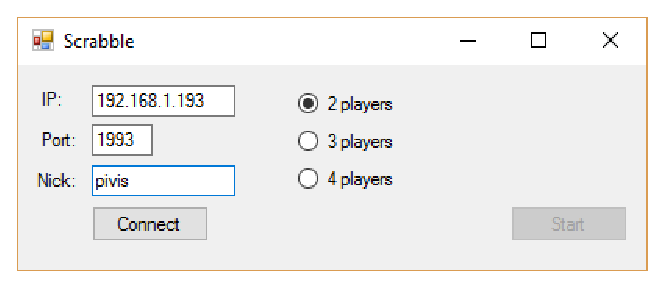
\includegraphics[width=0.5\textwidth]{img/main.eps}
	\caption{Přihlašovací okno}
  \label{main}
\end{figure}

Po připojení se do hry se kliknutím na tlačítko \emph{Start} zobrazí okno hry.

Odpojení se provede kliknutím na tlačítko \emph{Disconnect}.

\subsubsection{Ovládání hry}
Na hrací plán 15x15 (viz obr. \ref{game}) se umísťují písmena ze zásobníku. První písmeno musí být umístěno na středové pole. Samohlásky mají bodovou hodnotu 1, souhlásky 2 nebo 3 a písmeno Q, X nebo W hodnotu 10. Na hracím plánu jsou pole, která hodnotu písmene zdvojí (světle zelené), ztrojí (tmavě zelená) nebo zčtyřnásobí (červené). 

Po umístění všech písmen se tah ukončí kliknutím na tlačítko \emph{Turn}. Chybně umístěná písmena se dají vratit zpět do zásobníku. Tlačítko \emph{$<$} vrátí poslední umístěné písmeno, tlačítko \emph{Reset} se vrátí všechna písmena umístěná v daném tahu.

\begin{figure}[H]
	\centering
	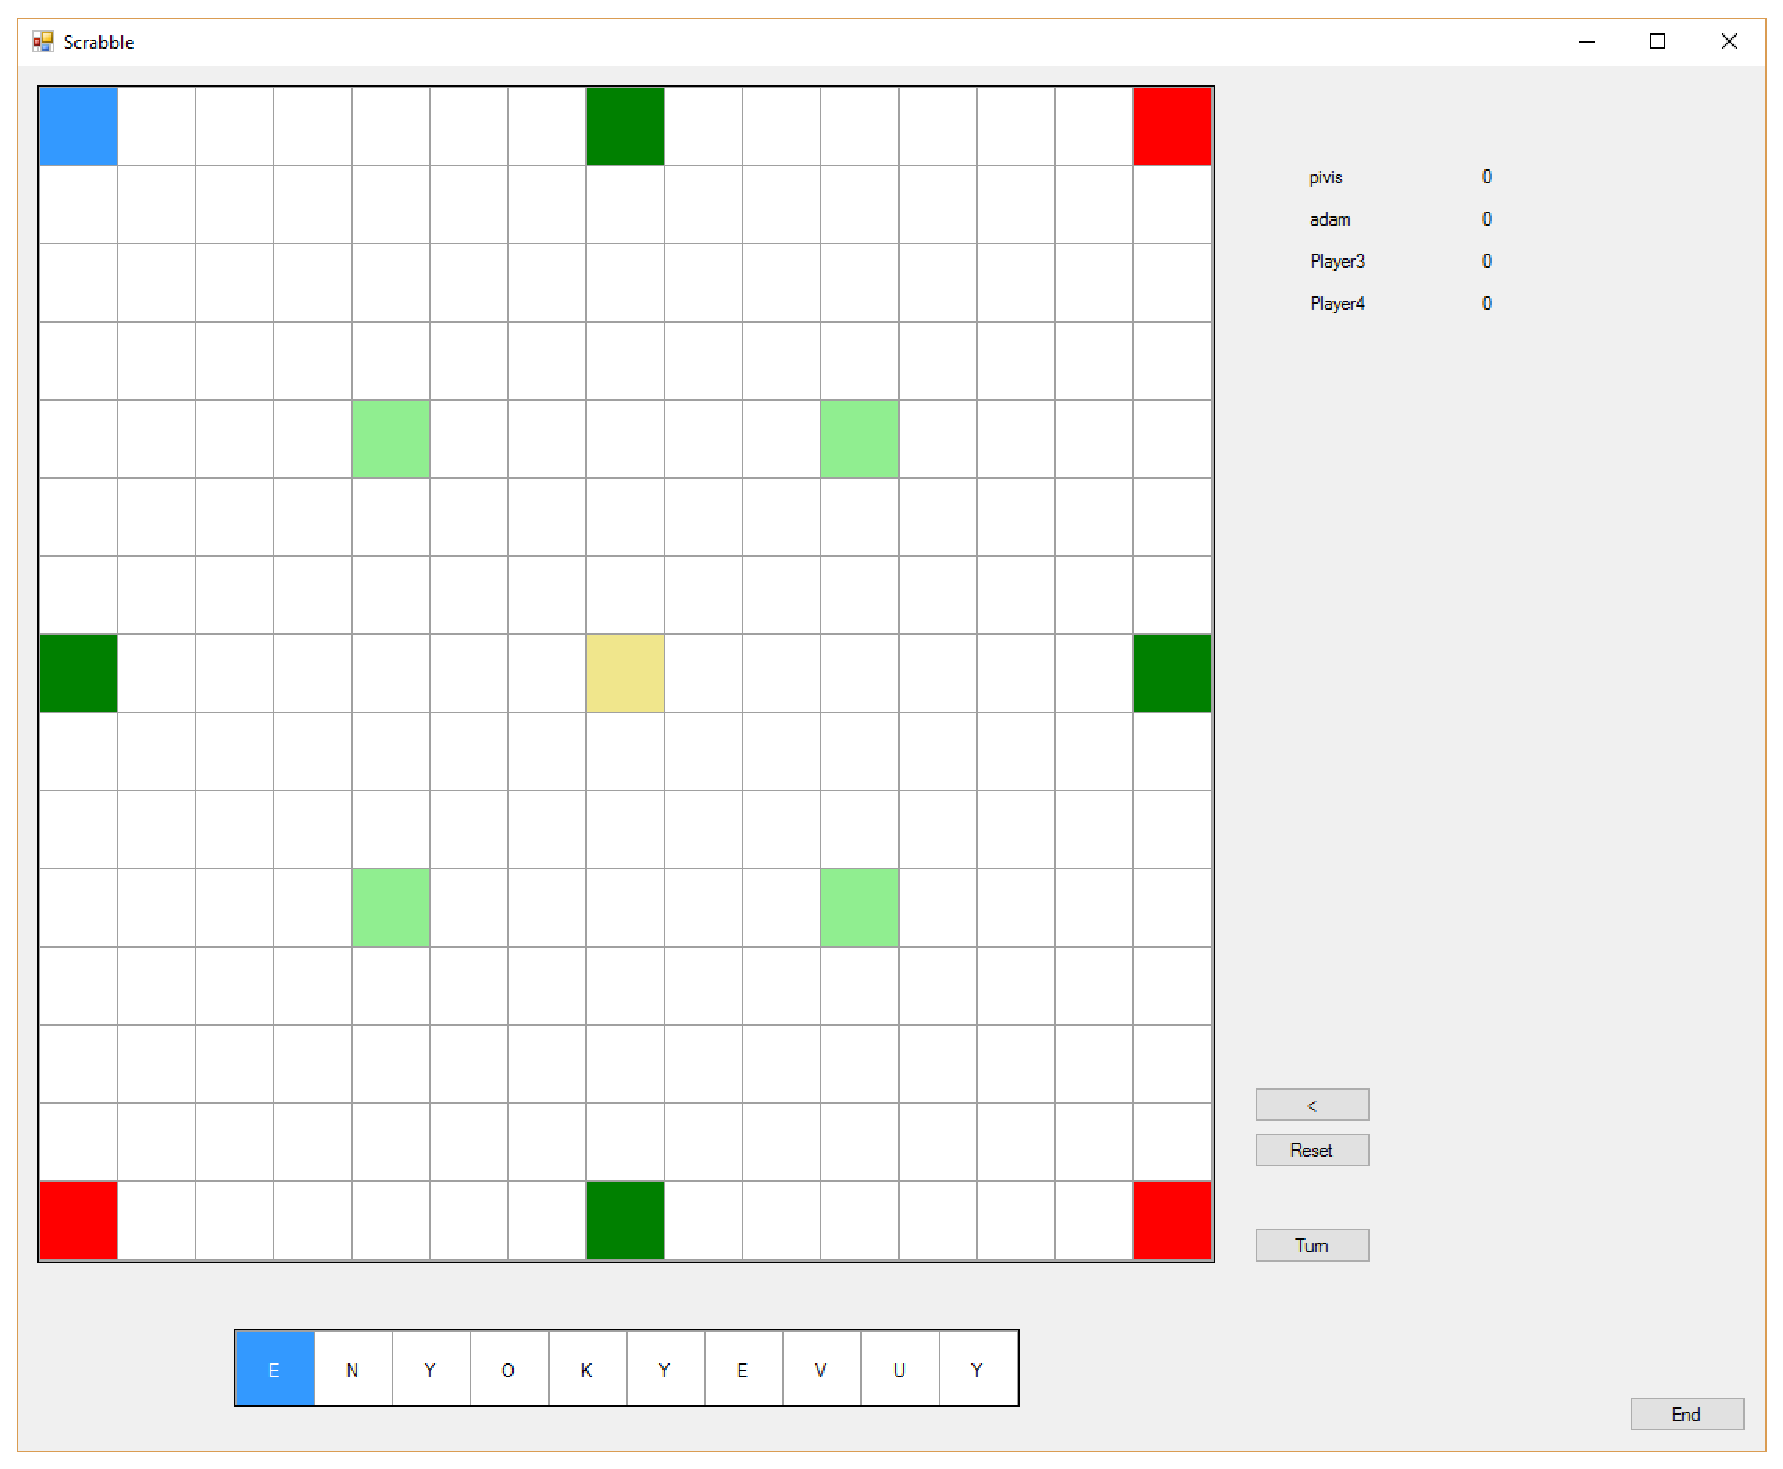
\includegraphics[width=0.8\textwidth]{img/game.eps}
	\caption{Okno hry}
  \label{game}
\end{figure}



\chapter{Závěr}
Práce splňuje zadání. Server umí obsluhovat více klientů současně a umožňuje hrát více her najednou. Také umožňuje znovu připojení hráče do probíhající hry. Klient je nezávislý na zpoždění síťových operací. Server i klient jsou schopni vyrovnat se s chybami a výpadky na síti.

Server i klienta lze spustit na operačním systému Linux a Windows.